% Mammografie links ohne, rechts mit Tumor; der rote Rahmen markiert den Befund
% (ersetzt das frühere Bild if-elif-else-cancer.jpg, dessen Quelle nicht belegt war).
% Bild: National Cancer Institute, gemeinfrei (PD-USGov), Wikimedia Commons "Mammo breast cancer.jpg".
\begin{tikzpicture}
	\node[anchor=south west, inner sep=0pt] (mammo) at (0,0)
	{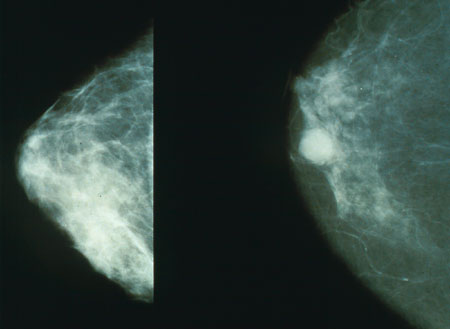
\includegraphics[height=3cm]{Grundlagen_Info/00_Programmieren/Figures/mammografie-nci.jpg}};
	% Koordinaten relativ zur Bildgrösse: (0,0) unten links, (1,1) oben rechts
	\begin{scope}[x={(mammo.south east)}, y={(mammo.north west)}]
		\draw[red, very thick] (.64,.47) rectangle (.77,.62);
	\end{scope}
	\node[anchor=north west, inner sep=0pt, text width=4.1cm, font=\tiny] at (mammo.south west)
	{\rule{0pt}{1.2em}Bild: National Cancer Institute, \href{https://commons.wikimedia.org/wiki/File:Mammo_breast_cancer.jpg}{Wikimedia Commons}, gemeinfrei};
\end{tikzpicture}
